\chapter{Systemarchitektur}
\begin{tiny}
MB
\end{tiny}
\section{Schichtenarchitektur}
	Die nachfolgende Figur soll die Schichtenarchitektur unseres Systems veranschaulichen. \\ \\
    %Bild der Schichtenarchitektur
    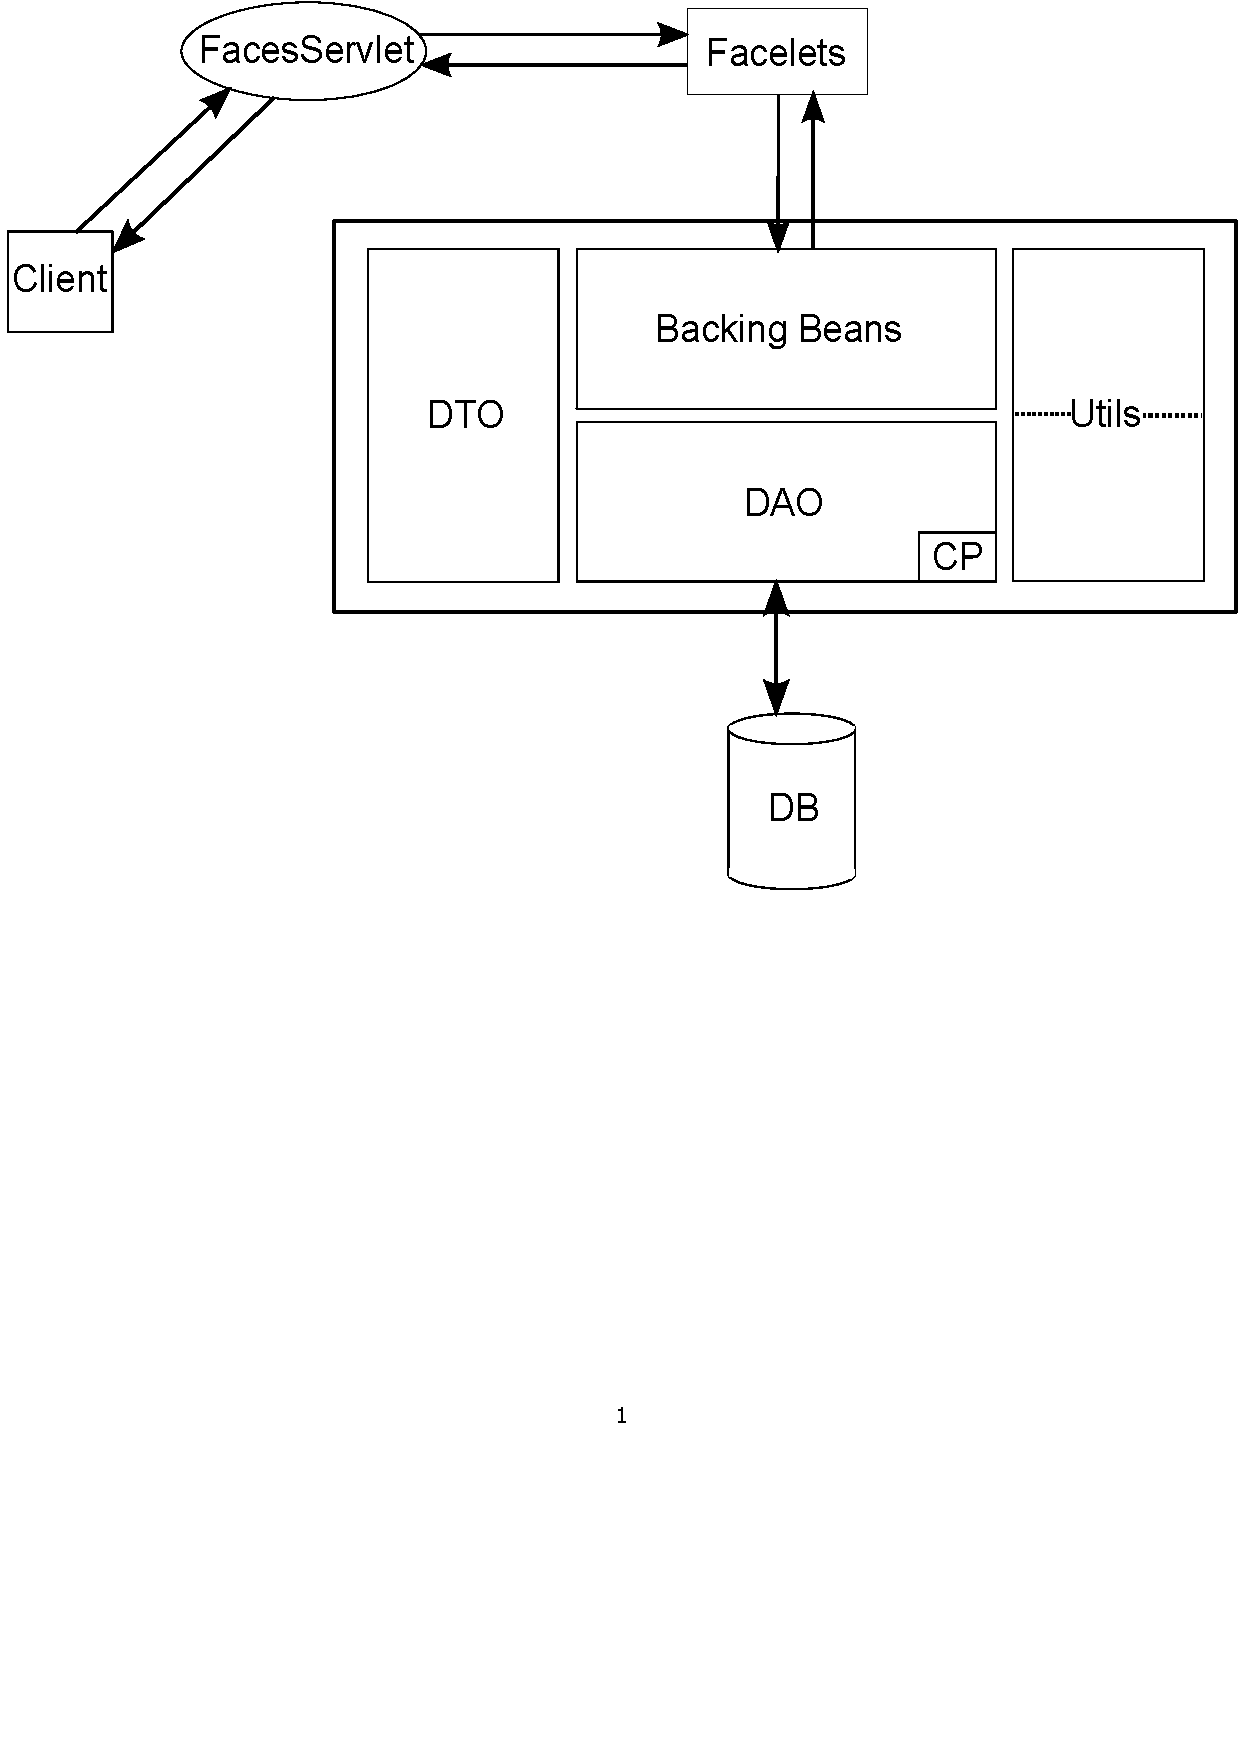
\includegraphics[scale=0.50]{Grafiken/Schichtenarchitektur.pdf}
	\subsection{Faces-Servlet}
	    Das Faces-Servlet fungiert im System als Controller, der eine HTTP-Request abfangt, diese bearbeitet, sowie weiterleitet. Das Faces-Servlet muss in jeder JSF-Applikation konfiguriert sein und wird in der web.xml Datei definiert. 
    \subsection{Facelets}
    	Die View wird durch Facelets repräsentiert. Es stellt den Inhalt dar, der vom Controller übergeben wird. Des Weiteren werden in der View die Benutzerinteraktionen entgegengenommen. Genauer auf Facelets wird unter Kapitel 4 Facelets eingegangen.
   	\subsection{Model}
   	Das Model kann in vier Bereiche unterteilt werden. Zunächst gäbe es die \glqq Upper Layer\grqq{}, welche die Backing Beans beinhalten, die \glqq Lower Layer\grqq{} mit den Data Access Objects (DAOs) und dem Connection Pool (CP), des Weiteren gäbe es noch die Data Transfer Objects (DTOs) und die Utils. 
   		\subsubsection{Upper Layer}
   		Die \glqq Upper Layer\grqq{} besteht aus den Backing Beans. In Diesen ist zum Einen die Geschäftslogik enthalten, zum Anderen werden dort die überlieferten Benutzereingaben der Facelets übergeben, weiterverarbeitet und gespeichert.
    	\subsubsection{Lower Layer}
    	In der \glqq Lower Layer\grqq{} befinden sich die Data Access Objects und der Connection Pool. Mithilfe des CP greifen die DAOs auf die darunterliegende Database (DB) zu.
    	\subsubsection{DTO}
    	Die Data Transfer Objects dienen als Schnittstelle zwischen den Backing Beans und den zugehörigen DAOs. Sie bündeln logisch zusammenhängende Daten in einem Objekt, um zeitintensive Fernzugriffe durch einen zu ersetzen.
    	\subsubsection{Utils}
    	Utils fungieren als Hilfs- und Verwalterklasse. Die Utils werden auch wiederum unterteilt, die man entweder den Backing Beans oder den DAOs zuordnen kann. 
    \subsection{Database}
    Die Database (DB) beinhaltet alle relevanten Daten, die für das System benötigt werden. Die DB kapselt die Daten von der Außenwelt ab, somit haben nur die DAOs haben Zugriff auf die DB. 
\section{Design Patterns}
Im Nachfolgendem werden die im System eingesetzten Design Patterns beschrieben:
	\begin{itemize}
		\item \textbf{Data Transfer Object:} Das DTO fassen mehrere Daten in einem Objekt zusammen, damit sie in einem Aufruf übergeben werden. Somit können Datensätze durch die Schichten transportiert werden.
		\item \textbf{Dependency Injection:} Dependency Injection ist ein JSF Standard, um Backing Beans zu verwalten. Hierbei werden die benötigten Objekte an einem zentralen Ort hinterlegt, was auch die Flexibilität erhöht.  
		\item \textbf{Creational Pattern:} Die Creational Pattern kann man wiederum in folgende Pattern unterscheiden.
			\begin{itemize}
				\item \textbf{Factory Pattern:} Hier werden mehrere ähnliche Objekte durch Aufruf einer Methode anstatt durch direkten Aufruf eines Konstruktors erzeugt.
				\item \textbf{Object Pooling:} Beim Object Pooling werden ressourcenintensive Objekte (hier Datenbankverbindungen) in einem Pool (Connection Pool) bereitgehalten, um sie bei Bedarf erneut nutzen zu können, was sich wiederum positiv auf die Ausführungszeit auswirkt.
				\item \textbf{Singleton:} Es soll sichergestellt werden, dass von einem Objekt jeweils nur eine Instanz existiert. Diese sind darüber hinaus global verfügbar.  
			\end{itemize}
	\end{itemize}
\section{Einsatz externer Libraries}
Es werden im System auf bereits vorhandenen Libraries zurückgegriffen.
	\begin{itemize}
		\item \textbf{PostgreSQL JDBC 9.4-1201:} Der PostgreSQL JDBC-Treiber wird für die Kommunikation mit der Datenbank verwendet.
		\item \textbf{JSF 2.2:} Für die Implementierung von JSF wird das Framework Mojarra 2.2.10 benutzt.
		\item \textbf{JavaMail API 1.5.2:} Library für das Versenden von Emails.
		\item \textbf{Bootstrap 3.3.0:} Bootstrap dient als Grundlage für das Design der Facelets.
		\item \textbf{Tomcat 8.0.21:} Webcontainer, um die in Java geschriebenen Webapplikationen auszuführen.
		\item \textbf{Commons Fileupload:} Library für das Hochladen von Dateien.
		\item \textbf{Log4J:} Library für das Loggen von Meldungen.
		\item \textbf{JFreeChart:} Library für die Erstellung von Diagrammen.  
	\end{itemize}
\section{Fehlerbehandlung}
	\subsection{Nicht-Autorisierter Zugriff}
	Sofern der User eine Aktion ausführen will, aber nicht die entsprechenden Rechte besitzt, wird eine Fehlermeldung ausgegeben (beispielsweise will ein Gast nach einem bestimmten Kurs suchen, was aber nur registrierte User vorbehalten ist) und der Gast wird gegebenenfalls auf die Login Seite verwiesen. Die Facelets werden mit einem Phaselistener überprüft.
	\subsection{Fehlerhafte Benutzereingaben}
	Wenn ein Gast sich registrieren will, aber in den Formulardaten ein ungültige Eingabe tätigt, so soll der Gast nicht alles neu eingeben müssen, sondern nur die fehlerhaften Stellen neu eingeben. Der Fehler wird auf derselben Seite angezeigt, somit wird keine Fehler-Seite extra benötigt.
	\subsection{Exceptions}
	Sollten Fehler auftreten auf die der User keinen Einfluss hat, so wird der Nutzer auf eine Fehler-Seite geleitet. Auf dieser Seite befinden sich Informationen zu dem Fehler und es wird eine weitere Vorgehensweise zur Verfügung gestellt. Bestimmte Exceptions wie beispielsweise eine SQL-Exception werden gefangen und geworfen, indem globale Exception-Handler implementiert werden. Bei kritischen Exceptions wird auch eine Logfile angefertigt, um im Nachhinein genau zu verfolgen wo und wann der Fehler aufgetreten ist.
	\subsection{HTTP-Statuscodes}
	Für den User werden in der web.xml HTTP-Statuscodes generiert. Somit bleiben kryptische Fehlermeldungen seitens des Webservers dem User verborgen. Dem User werden die Fehler auf einer neuen Seite angezeigt: \\ \\
	\begin{tabular}{|l|l|}
		\hline
		Status Code & Beschreibung \\
		\hline
		403 & Zugriff nicht autorisiert \\
		404 & Datei/Ressource nicht vorhanden \\
		408 & Server-Timeout \\
		500 & Interner Server Fehler \\
		503 & Server nicht erreichbar \\
		\hline
 	\end{tabular}		     

